\documentclass[12pt]{extarticle}

\usepackage[utf8]{vietnam}
\usepackage{graphicx}
\usepackage{fancyhdr}
\usepackage{parskip}
\usepackage{amssymb}
\usepackage{amsmath}
\usepackage{tikz}
\usepackage{fancybox}
\usetikzlibrary{positioning}
\usepackage[left=3 cm,right=2 cm,top=3cm,bottom=3cm]{geometry}
\usepackage[labelfont=bf]{caption}
\usepackage[bookmarks=true]{hyperref}
\usepackage{bookmark}


\pagestyle{fancy}
\fancyhf{}

\rhead{Dự đoán mức độ thu hút của địa điểm ăn uống trong tương lai}
\fancyfoot[LE,RO]{\thepage}
\renewcommand{\headrulewidth}{0.4pt}
\renewcommand{\footrulewidth}{0.4pt}

\graphicspath{{images/}}
%\title{Báo cáo Thực tập tốt nghiệp\\Đề tài: Dự đoán mức độ thu hút của địa điểm ăn uống trong tương lai}
%\date{17-5-2016}
%\author{GVHD: GS.TS Cao Hoàng Trụ \\\\ Nguyễn Trọng Nghĩa \texttt{51202370}
% \\ Nguyễn Đăng Trang \texttt{51203957}}

\begin{document}

%Title Page
\begin{titlepage}
	\thispagestyle{empty}
	\thisfancypage{
	\setlength{\fboxsep}{0pt}
	\fbox}{} 
	\begin{center}
		\begin{large}
			TRƯỜNG ĐẠI HỌC BÁCH KHOA THÀNH PHỐ HỒ CHÍ MINH
		\end{large} \\	
		\begin{large}
			KHOA KHOA HỌC \& KỸ THUẬT MÁY TÍNH
		\end{large} \\
		\textbf{---------------------------------------------}\\[1cm]

		\begin{figure}[h!]
			
\includegraphics{logo}
			\centering
		\end{figure}

		\vspace{1cm}

		{\fontsize{40pt}{1}\selectfont BÁO CÁO THỰC TẬP TỐT NGHIỆP}\\
		{\fontsize{20pt}{1}\selectfont ĐỀ TÀI: DỰ ĐOÁN MỨC ĐỘ THU HÚT \\ CỦA ĐỊA ĐIỂM ĂN UỐNG TRONG TƯƠNG LAI}\\[3cm]
	\end{center}

	\hspace{2cm} Sinh viên thực hiện : \hspace{16pt}
	\textbf{\parbox[t]{7cm}{    
		Nguyễn Đăng Trang \hspace{4pt}51203957 \\
		Nguyễn Trọng Nghĩa 51202370
	}}\\[12pt]

	\hspace{2cm} Giảng viên hướng dẫn :  \hspace{3pt} \textbf{\parbox[t]{5cm}{    
		GS.TS Cao Hoàng Trụ
	}}

	\vspace{2cm}
	\begin{center}
		{\fontsize{14pt}{1}\selectfont Thành phố Hồ Chí Minh}\\
		{\fontsize{14pt}{1}\selectfont \today}
	\end{center}


\end{titlepage}


% Vẽ hình
	\tikzset{%
	  every neuron/.style={
   	 circle,
   	 draw,
   	 minimum size=1cm
  	},
 	 neuron missing/.style={
  	  draw=none, 
  	 scale=3,
   	 text height=0.333cm,
    	execute at begin node=\color{black}$\vdots$
  	},
	}
	\pagenumbering{gobble}
%	\maketitle
	\newpage
	\thispagestyle{empty}
	\pdfbookmark{\contentsname}{Mục lục}
	\tableofcontents
	\pagenumbering{arabic}
	\newpage
  	\addcontentsline{toc}{section}{Danh sách hình vẽ}
	\listoffigures
	\newpage
	\addcontentsline{toc}{section}{Danh sách bảng}
	\listoftables
	\newpage
	\section{Tóm tắt báo cáo}	
		\par Bài báo cáo trình bày về chủ đề Phân tích dữ liệu trên mạng xã hội (MXH) và đi sâu vào một bài toán dùng học máy phân tích dữ liệu trên MXH do nhóm đề xuất, gồm ba phần:
		\begin{itemize}

		\item{Phần đầu nói khái quát về MXH và những vấn đề nghiên cứu trên MXH.}	

		\item{Phần tiếp theo dẫn dắt vào đề tài mà nhóm đề xuất, đó là bài toán về Dự đoán mức độ thu hút của địa điểm ăn uống trong tương lai. Nghiên cứu thu hẹp lại trên các MXH về địa điểm ăn uống, bài báo cáo nêu lên các nghiên cứu liên quan đến các MXH về địa điểm ăn uống và liên quan đến bài toán được đề xuất.}

		\item{Các phần còn lại trình bày kiến thức nền tảng liên quan được sử dụng trong phương pháp đề xuất và đưa ra phương pháp đề xuất.}


		\end{itemize}

	\section{Khái quát về MXH và Phân tích dữ liệu trên MXH}
		\subsection{Khái quát về MXH}
			\par Sự bùng nổ của công nghệ thông tin và sự phổ biến rộng rãi của các thiết bị có khả năng kết nối Internet, đặc biệt là các thiết bị di động như điện thoại thông minh, máy tính bảng đã tạo điều kiện cho các MXH trực tuyến phát triển nhanh chóng.
			\par Các MXH trực tuyến như \textit{Facebook}, \textit{Twitter} , \textit{Flickr}, \textit{Foody} … dần trở thành một phần quan trọng trong cuộc sống của mỗi cá nhân.
			\begin{itemize}
				\item{Nó giả lập những yếu tố thực tế của xã hội con người mà ở đó người dùng có thể nói chuyện, đăng bài, kết bạn, đặt relationship … (\textit{Facebook}, \textit{Twitter})}	
				\item{Nó cung cấp cho người dùng sự tiện lợi về một nhu cầu nào đó (\textit{Flickr} – chia sẻ ảnh, \textit{Foody}  – chia sẻ địa điểm ăn uống)}
			\end{itemize}

			\par Một MXH có thể được hiểu như là một hệ thống mà chức năng chính là cho phép người dùng thực hiện các tương tác xã hội trên đó (\textit{Facebook}, \textit{Twitter}) hoặc là một hệ thống phục vụ chức năng khác (\textit{Flickr} – chia sẻ ảnh, \textit{Foody}  – chia sẻ thông tin địa điểm ăn uống) nhưng vẫn cho phép người dùng thực hiện những tương tác nhất định trên đó. 
			\par Nói một cách tổng quát, MXH là một mạng của các tương tác và mối quan hệ, mà trong mạng đó các nốt (node) đại diện cho các tác nhân và các cạnh (edge) đại diện cho các tương tác hoặc mối quan hệ giữa các tác nhân đó. Điều này có nghĩa là khái niệm MXH không chỉ bị giới hạn trong những trang MXH trực tuyến như \textit{Facebook}, \textit{Foody} … mà tổng quát hơn, nó là mạng của bất cứ các tác nhân nào tương tác với nhau, tương tác này có thể được thực hiện qua mạng Internet, qua thư bưu chính hay mặt đối mặt.

		\subsection{Khái quát về Phân tích dữ liệu trên MXH}
			\par Một khía cạnh rất quan trọng khi xét đến các MXH trực tuyến là chúng chứa lượng dữ liệu khổng lồ, cho phép nghiên cứu trên đó nhằm tìm ra các đặc điểm của MXH, đặc điểm của các tác nhân (actor) trên MXH hay đặc điểm các mối liên kết giữa các tác nhân này.

			\par Có hai hướng phân tích dữ liệu trên MXH trực tuyến [1], đó là:
			\begin{itemize}
				\item{Phân tích dữ liệu dựa trên cấu trúc và liên kết (Linkage-based and Structural Analysis): Gồm các nghiên cứu về \textit{Hành vi lan truyền, Phát hiện cộng đồng, Xác định các tác nhân quan trọng trong MXH, Dự đoán liên kết, Niềm tin trên MXH, Phân loại nốt} và \textit{Tìm kiếm chuyên gia trên MXH}}	
				\item{Phân tích dữ liệu dựa trên nội dung người dùng đưa lên (Content-based Analysis): Lượng dữ liệu khổng lồ mà người dùng đưa lên trên các trang MXH như \textit{Facebook}, \textit{Youtube}, \textit{Flickr} (hình ảnh)… là cơ sở cho việc nghiên cứu kết hợp với các phân tích liên quan đến cấu trúc và liên kết nhằm tìm ra những đặc điểm của MXH.}
			\end{itemize}
			\par Để hiểu hơn về các thành phần của MXH, về dữ liệu trên MXH và những nghiên cứu trong việc phân tích các dữ liệu này, nhóm trình bày một số vấn đề nghiên cứu và bài toán quan trọng trong Phân tích dữ liệu MXH ở hai mục tiếp theo. Mục 2.3 trình bày các chủ đề nghiên cứu về Phân tích dữ liệu dựa trên cấu trúc và liên kết; mục 2.4 trình bày các chủ đề nghiên cứu về Phân tích dữ liệu dựa trên nội dung người dùng đưa lên.
			\subsection {Phân tích dữ liệu dựa trên cấu trúc và liên kết}
			\par \textbf{Hành vi lan truyền (Cascading Behavior)}
			\par \textit{Hành vi lan truyền} là nghiên cứu việc phát hiện và theo dõi một “xu hướng” mới trên MXH. Khi một người nào đó post một bài viết hay, hoặc một sự kiện xảy ra, một sản phẩm được ra mắt, ban đầu nó không được chú ý nhiều; nhưng dần dần, theo ảnh hưởng của người dùng, mọi người bắt đầu quan tâm, bàn luận đến vấn đề đó. Khi đó, vấn đề đó trở thành một “xu hướng” hay “trào lưu” mới trong MXH. \textit{Hành vi lan truyền} khác với \textit{Phát hiện sự kiện} ở chỗ sự kiện diễn ra ngoài đời thực được nhiều người biết đến và đưa nó lên MXH, còn “trào lưu” thì sinh ra và lan truyền trên MXH. Vậy điều quan trọng trong chủ đề này là làm thế nào để xác định được “xu hướng” mới và theo dõi sự lan truyền của nó. “Xu hướng” được lan truyền qua những đối tượng trong MXH, dựa vào sự lan truyền ấy có thể đánh giá đối tượng nào có ảnh hưởng lớn đối với sự lan truyền trong MXH.
			\par Nghiên cứu về \textit{Hành vi lan truyền} có thể giúp tìm kiếm, phát triển các ý tưởng mới trên mạng xã hôi; giúp cho lĩnh vực truyền thông trong việc phát hiện, theo dõi các “xu hướng” mới hoặc ứng dụng để gợi ý, thông báo “trào lưu” mới cho người dùng.
			\par \textbf{Phát hiện cộng đồng (Communty Discovery)}
			\par \textit{Cộng đồng (community)} trong MXH là tập hợp một nhóm người dùng có chung một đặc điểm nào đó, \textit{ví dụ}: sở thích, hay cùng mối quan tâm, …  Một cộng đồng gồm chủ đề (theme) và tập hợp người dùng trong cộng đồng đó. Chủ đề là điểm chung mà người trong cộng đồng quan tâm.
			\par \textit{Phát hiện cộng đồng} trong MXH gồm 2 yêu cầu là xác định chủ đề và tập hợp người dùng trong cộng đồng đó. Một vấn đề nghiên cứu quan trọng trong chủ đề này là nghiên cứu về “sự thay đổi” của cộng đồng theo thời gian: việc thay đổi về kích thước cũng như các giai đoạn của một cộng đồng. \textit{Ví dụ}: khi nào một cộng đồng mới được hình thành hoặc tan rã, một cộng đồng bị tách ra làm 2 cộng đồng nhỏ, 2 cộng đồng hợp lại làm một. 
			\par Việc nghiên cứu để phát hiện cộng đồng thuộc một lĩnh vực cụ thể có thể cung cấp những thông tin hữu ích, cập nhật đối với những người dùng quan tâm đến lĩnh vực đó. Mặt khác, nó là nền tảng cho các nghiên cứu trên web liên quan đến cộng đồng, đặc trưng của cộng đồng và nó giúp cho việc quảng cáo được hiệu quả khi nội dung quảng cáo dựa trên chủ đề/lĩnh vực quan tâm của cộng đồng.
			\par \textbf{Xác định tác nhân quan trọng trong MXH (Identifying prominent actors in social network)}
			\par \textit{Những người nổi bật trong MXH} là những người có vai trò trung tâm, có liên hệ với nhiều người khác. Trong ngữ cảnh một tổ chức/cộng đồng, những người này được xem là có vai trò quan trọng hơn nhiều so với những người ít giao tiếp quan hệ với người xung quanh.
			\par Khi mô hình hóa MXH bằng đồ thị, ta có thể hình dung đơn giản rằng những người nổi bật sẽ được thể hiện bằng những đỉnh có số lượng đỉnh liền kề lớn. Có nhiều thang đo để đánh giá sự nổi bật của một người trong MXH, trong đó đáng chú ý nhất là \textit{Rank Prestige}. Giải thuật xếp hạng kết quả tìm kiếm (\textit{PageRank}) của \textit{Google} được hiện thực dựa trên \textit{Rank Prestige} và đã biến \textit{Google} thành công cụ tìm kiếm đứng đầu thế giới.
			\par Vấn đề cần nghiên cứu chủ yếu trong chủ đề này là đánh giá các người dùng trong MXH để tìm ra người nổi bật nhất (có thể ứng dụng giải thuật \textit{PageRank} hoặc các biến thể của nó). Nghiên cứu này mang nhiều ý nghĩa thực tế. \textit{Ví dụ}: trong lĩnh vực marketing, có thể tìm hiểu những đối tượng nào có khả năng thu hút cộng đồng MXH lớn để truyền thông tin, quảng bá.
			\par \textbf{Dự đoán liên kết (Link prediction)}
			\par \textit{Dự đoán liên kết} nghiên cứu về mối quan hệ (liên kết) giữa các tác nhân (actor) trong MXH. Nó được chia làm 3 bài toán cụ thể: dự đoán những mối quan hệ tồn tại trong MXH hiện tại mà ta không thể thu thập được; dự đoán những mối quan hệ sẽ hình thành trong MXH tương lai; dự đoán những mối quan hệ sẽ kết thúc trong MXH tương lai.
			\par Vấn đề khai thác MXH hiện nay đối mặt hai thách thức. Thách thức thứ nhất là dữ liệu không đầy đủ (incompletion): Phần lớn dữ liệu về MXH thu thập được không đầy đủ bởi vì chỉ một phần thông tin MXH có thể thu thập được từ các ứng dụng thu thập dữ liệu MXH. Thách thức thứ hai đó là dữ liệu thay đổi liên tục (Dynamic): MXH có đặc trưng là luôn thay đổi liên tục, do đó mỗi đỉnh hay cạnh có thể xuất hiện và biến mất liên tục.
			\par Một số ứng dụng của \textit{Dự đoán liên kết} trên MXH:
			\begin{itemize}
				\item Gợi ý trên MXH, điển hình là gợi ý bạn bè, đồng nghiệp, người theo dõi (follower) và người được theo dõi (followee).
				\item Giải quyết vấn đề hoàn chỉnh mạng. Mục đích của vấn đề là suy luận tìm ra những nốt và liên kết bị thiếu trong quá trình thu thập thông tin.
				\item Dự đoán mối quan hệ xã hội. \textit{Ví dụ}: dự đoán mức độ mối quan hệ (mạnh hay yếu) và mô hình mức độ quan hệ đó. Mặc dù nó không liên quan trực tiếp đến dự đoán liên kết, nhưng những kết quả của nó có thể dẫn đến những phương pháp dự đoán liên kết mới.
				\item Ứng dụng vào các lĩnh vực khác. \textit{Ví dụ}: trong sinh học, dự đoán tương tác protein-protein. 
			\end{itemize}
			\par \textbf{Niềm tin trên MXH (Trust in social network)}
			\par \textit{Niềm tin trên MXH} là lòng tin giữa người dùng trong MXH. Trên MXH, các người dùng có thể không biết nhau ngoài đời thật, nên cần có một công cụ để đánh giá lòng tin giữa các người dùng với nhau, giúp đánh giá về thông tin đăng trên MXH cũng như về bản thân một người dùng (hay tổ chức/công ty) tham gia vào MXH.
			\par Lòng tin rất khó định nghĩa, ngay cả ở ngoài đời thực. Lòng tin bị ảnh hưởng bởi rất nhiều nhân tố, cả về tâm lí, xã hội,.. nên khó có thể đo được chính xác. Hai điểm lưu ý trong vấn đề lòng tin giữa đời thực và MXH: sự khác nhau giữa văn hóa, quan điểm, thể chế giữa các người dùng trong MXH là rất nhiều; danh tính của một người trên MXH có thể không phản ánh đúng như ở ngoài đời thật.
			\par Một số vấn đề nghiên cứu trong chủ đề này: định nghĩa lòng tin trong MXH; tìm một thước đo hợp lí về lòng tin và các nhân tố ảnh hưởng đến lòng tin; mô hình hóa một hệ thống biểu diễn lòng tin giữa các người dùng trong MXH; đánh giá mức độ tin tưởng giữa 2 người dùng chưa hề có mối quan hệ nào dựa vào mô hình lòng tin đã biết trước.
			\par \textit{Niềm tin trên MXH} có nhiều ứng dụng quan trọng, bao gồm: giúp đánh giá mức độ tin cậy của một thông tin hay người dùng trên MXH; giúp các công ty/tổ chức nâng cao được lòng tin với khách hàng và giúp đánh giá, gợi ý kết bạn cho người dùng.
			\par \textbf{Phân loại nốt (Node classification)}
			\par Mỗi người dùng trong MXH có rất nhiều thông tin: hồ sơ người dùng (profile), các hoạt động tương tác, bình luận, status, các group tham gia. Những thông tin này được phân loại và gán nhãn, \textit{ví dụ}: từ thông tin tuổi gán nhãn cho người đó là trẻ, từ quan hệ tình cảm có thể gán nhãn là độc thân, kết hôn hay đã li dị,.. Mỗi người sẽ có nhiều nhãn dựa vào thông tin của họ.
			\par Bài toán đặt ra cho phân loại nhãn đó là: trong MXH, khi đã biết nhãn tương ứng với một vài người, làm sao gán nhãn cho những người dùng còn lại dựa vào các tương tác giữa họ với những người đã biết; ngoài ra, có thể đánh giá mức độ liên hệ giữa các nhãn với một người dùng.
			\par Trong cách phân loại truyền thống, việc nghiên cứu chỉ dựa trên các thuộc tính của một người dùng để gán nhãn cho họ. Ngược lại trong MXH, việc phân loại một người dùng còn bị ảnh hưởng bởi mối quan hệ giữa người dùng đó với các người dùng khác.
			\par Một vài ứng dụng quan trọng của \textit{Phân loại nốt} là: xây dựng hệ thống gợi ý đến người dùng (âm nhạc, phim ảnh, bạn bè,…) dựa trên nhãn mà người dùng được gán; hệ thống hỏi đáp mà những câu hỏi sẽ được trực tiếp gửi đến các chuyên gia có thể trả lời hợp lý; hệ thống quảng cáo: dựa trên việc gán nhãn người dùng, người quảng cáo có thể đưa ra quyết định nhanh chóng có nên quảng với người đó hay không.
			\par \textbf{Tìm kiếm chuyên gia trên MXH (Expert finding in Social Network)}
			\par \textit{Tìm kiếm chuyên gia trên MXH} là một trong những chủ đề nghiên cứu quan trọng trong MXH. Mục tiêu của chủ đề này là nhằm tìm kiếm những người trên MXH có kiến thức hay kinh nghiệm về một đề tài nhất định, chẳng hạn như toán học, vật lý, công nghệ,… Những người này có vai trò quan trọng vì họ có khả năng chia sẻ, truyền đạt những kiến thức, kinh nghiệm của mình cho những người khác quan tâm đến chủ đề đó.
			\par Trong chủ đề này, ta cần nghiên cứu về thông tin cá nhân của mọi người trên MXH và những mối liên hệ giữa người với người. Ta sử dụng những thông tin cá nhân để đánh giá “điểm chuyên gia” cho mọi người và dùng số điểm này để xếp hạng, rồi chọn ra những người có số điểm cao nhất làm ứng cử viên. Các ứng cử viên này sẽ được dùng để xây dựng đồ thị. Sau đó, sử dụng mối quan hệ của các ứng cử viên với các chuyên gia (cho trước) để tìm ra những ứng cử viên có thể là chuyên gia.
			\par Ứng dụng của các nghiên cứu trên chủ đề này có thể kể tới là: với một lĩnh vực nhất định, xác định các người dùng có ảnh hưởng để giúp marketing doanh nghiệp; hoặc gợi ý cho người dùng về những chuyên gia trong lĩnh vực họ hứng thú.
			
			\subsection {Phân tích dữ liệu dựa trên nội dung người dùng đưa lên MXH}
			\par Người dùng có thể đưa lên các trang MXH một lượng dữ liệu khổng lồ. Các nội dung này cho phép người dùng chia sẻ quan điểm cá nhân, ý kiến cá nhân và là phương tiện để tương tác trên MXH.
			\par Có thể thấy dữ liệu trên các trang MXH rất đa dạng về định dạng: hình ảnh, video, văn bản … \textit{Ví dụ}: \textit{Flickr} cho phép người dùng chia sẻ hình ảnh chất lượng cao và kèm theo các mô tả, \textit{Youtube} là trang chia sẻ video kèm theo các mô tả và cho phép người dùng bình luận lên đó, \textit{Facebook} cho phép người dùng đăng các post không những chứa dữ liệu dạng văn bản mà có thể kèm theo cả hình ảnh, video.
			\par Dữ liệu ở dạng văn bản đóng vai trò quan trọng trong các trang MXH. Đối với những trang MXH như \textit{Facebook}, \textit{Twitter} dữ liệu dạng văn bản được thể hiện qua những bài post và những bình luận của người dùng trên những bài post đó. Đối với những trang MXH mà chủ thể là hình ảnh hoặc video như \textit{Flickr} hay \textit{Youtube}, thì dữ liệu ở dạng văn bản cũng đóng vai trò quan trọng. Nó được dùng để mô tả cho chủ thể hoặc là nội dung phần bình luận của người dùng.
			\par Do đó việc khai phá dữ liệu dạng văn bản là rất hữu ích và có nhiều ứng dụng quan trọng. Khai phá dữ liệu dạng văn bản (Text Mining) có thể hiểu là việc khám phá tri thức được ẩn sau các dữ liệu dạng văn bản. Nó liên quan đến nhiều lĩnh vực khác như Học máy, Xử lý ngôn ngữ tự nhiên, Khai phá dữ liệu.
			\par Quá trình Khai phá dữ liệu dạng văn bản có thể được tóm tắt qua 3 giai đoạn:
			\begin{itemize}
				\item Tiền xử lý (Text preprocessing): làm sạch và tạo ra đầu vào phù hợp cho giai đoạn Biểu diễn .
				\item Biểu diễn (Text Presentation): mô hình hóa dữ liệu. Một cách thông dụng để thực hiện mô hình hóa là chuyển đổi dữ liệu đã tiền xử lý thành dạng vector số. Dưới dạng vector số, ta có thể thực hiện các phép toán đại số tuyến tính lên nó (Dạng biểu diễn này được gọi là Bag of Words hay Vector Space Model).
				\item Khám phá tri thức (Knowledge Discovery): áp dụng các kỹ thuật trong Học máy, Khai phá dữ liệu và Xử lý ngôn ngữ tự nhiên lên dạng Biểu diễn để tìm ra thông tin cần thiết.
			\end{itemize}
			\par Kết quả của quá trình Khai phá sẽ cung cấp những thông tin cần thiết cho người dùng. Tuy nhiên, dữ liệu dạng văn bản trên MXH có những đặc trưng riêng và chúng là thách thức cho việc khai phá này. Những đặc trưng đó là: Tính nhạy cảm theo thời gian, Tính ngắn gọn, Tính phi cấu trúc và Tính phong phú về thông tin. Cụ thể:
			\begin{itemize}
				\item Tính nhạy cảm theo thời gian (Time Sensitivity): dữ liệu trên các trang MXH được cập nhật từng phút. Các người dùng khác nhau trên \textit{Twitter} hay \textit{Facebook} đăng các post hoặc bình luận hàng giờ, hàng phút để tương tác với những người dùng khác. Do đó dữ liệu trên các trang MXH được cập nhật nhanh chóng theo thời gian. Việc truy vấn thông tin từ dữ liệu của các MXH ở thời điểm hiện tại đôi khi cho ra những kết quả đã cũ của nhiều phút trước.  
				\item Tính ngắn gọn (Short Length): Các trang MXH thường có giới hạn nhất định về độ dài của các bài post, bình luận hay review. \textit{Ví dụ}: \textit{Twitter} giới hạn bài post tối đa 140 ký tự, \textit{Picasa} giới hạn bình luận tối đa 512 ký tự. Sự ngắn gọn này là thách thức đối với các kỹ thuật khai phá truyền thống trên dạng dữ liệu văn bản.
				\item Tính phi cấu trúc (Unstructured Phrases):
					\begin{itemize}
						\item Chất lượng của nội dung được biểu đạt qua một đoạn dữ liệu dạng văn bản không giống nhau tùy thuộc vào người viết. \textit{Ví dụ}: đối với cùng một địa điểm ăn uống trên \textit{Foody}, một người có kinh nghiệm ăn uống sẽ viết một bài review “hay” so với một người chưa có kinh nghiệm.
						\item Do những đặc trưng riêng của MXH, nội dung các bài post, bình luận, review thường chứa những tiếng lóng, từ viết tắt thiếu ngữ nghĩa … gây khó khăn cho các kỹ thuật phân tích. Ví dụ về một bình luận trên \textit{Foody}: “\textit{Hqua mình k ăn món cá ở đó}”.
					\end{itemize}
				\item Tính phong phú về thông tin (Abundant Information): Dữ liệu dạng văn bản trên MXH có thể tồn tại dưới nhiều hình thức và mang những ý nghĩa khác nhau. \textit{Ví dụ}: Một bài post trên \textit{Facebook} có nội dung chính là câu “\textit{Du lịch miền Tây}”, nó đi kèm với hashtag \textit{\#mientay} và một bức ảnh, trong đó mỗi phần của bức ảnh tag tên của những người dùng là bạn bè của người đăng. Những hình thức như hashtag hay tag hình ảnh trong \textit{Facebook} cho phép dữ liệu dạng văn bản mang thông tin liên quan đến liên kết giữa các nốt trong mạng.
			\end{itemize}
			\par \textit{Những chủ đề trình bày sau đây là các ứng dụng của Khai phá dữ liệu dạng văn bản trên MXH trực tuyến}.
					
			\par \textbf{Hệ thống hỏi đáp (Questioning \& Answer - QA)}
			\par Một lượng lớn các câu hỏi và câu trả lời của người dùng xuất hiện hằng ngày trên các trang hỏi đáp (QA) như \textit{Yahoo! Answer}, \textit{Quora} hay \textit{StackOverFlow}… Các trang QA này cũng là các MXH, nơi mà người dùng có thể đặt câu hỏi và tìm kiếm câu trả lời cho các câu hỏi mà mình mong muốn, đồng thời thu thập các ý kiến về một vấn đề nhất định hoặc tương tác với các người dùng khác ở đó. 
			\par Theo thời gian, số lượng các câu hỏi và câu trả lời trên các trang QA trở nên rất lớn và tạo nên cơ sở dữ liệu của riêng nó, do đó thay vì tìm kiếm các document từ web hoặc post một câu hỏi mới trên các forum, người dùng có thể vào các trang QA này và tìm câu trả lời cho các vấn đề quan tâm.
			\par Một số vấn đề được đặt ra trên các trang QA: thứ nhất, khi người dùng lên các trang QA để thực hiện truy vấn nhằm tìm kiếm một vấn đề quan tâm, làm thế nào để tìm ra các cặp QA đã có trên trang đó phù hợp với truy vấn mà người dùng thực hiện; thứ hai, tương ứng với mỗi \textit{Question} trong các cặp QA được tìm ra, tìm ra các \textit{Answer} tốt nhất.
			\par \textbf{Gán nhãn trên MXH (Social Tagging)}
			\par Người dùng có thể đưa các thực thể khác nhau (ảnh, audio, văn bản…) lên MXH và đính kèm theo nó các từ khóa (keyword) để mô tả, gán nhãn cho nội dung chính. Những từ khóa này là một hình thức của \textit{Gán nhãn trên MXH}. Việc gán nhãn này có nhiều ứng dụng trên MXH:
			\begin{itemize}
				\item Tìm kiếm dựa trên nhãn (tag): Người dùng trên các trang MXH có thể tìm kiếm các thực thể được gán nhãn tương tự hoặc liên quan ngữ nghĩa đến nhãn mà họ đem tìm kiếm. Vấn đề đặt ra là làm sao có thể tìm được các thực thể liên quan ngữ nghĩa này. \textit{Ví dụ}: khi người dùng tìm kiếm về một sự kiện gần đây, như “\textit{Cuộc cách mạng Ai Cập}”, hệ thống chỉ trả về các kết quả có nhãn là “\textit{Cuộc cách mạng}” và “\textit{Ai Cập}”, những thông tin về các nhãn khác như “\textit{Mubarak từ chức}” hay “\textit{Phản đối}” mặc dù có liên quan đến nhãn “\textit{Cách mạng Ai Cập}” bị bỏ qua. Hiện tượng này là do sự “thiếu ngữ nghĩa” trong việc xử lí nhãn, nguyên nhân là nhãn quá ngắn.
				\item Gợi ý nhãn (tag recommendation): Khi người dùng đưa một thực thể (ảnh, audio, văn bản, …) lên MXH trực tuyến, hệ thống sẽ đưa ra gợi ý cho người dùng những nhãn nào là phù hợp nhất cho thực thể đó. Vấn đề đặt ra là làm thế nào để tạo ra một hệ thống gợi ý có hiệu quả.   
				\item Phân loại các thực thể trên mạng (web objects classification): Cùng với sự bùng nổ của mạng xã hội nơi người dùng có thể đưa lên hàng triệu video, hình ảnh… mỗi giờ, sự phát triển nhanh chóng về số lượng và chủng loại của các thực thể này đặt ra yêu cầu cần thiết phải phân loại chúng một cách hiệu quả. Trên MXH, người dùng được cho phép gán nhãn (tag) cho các thực thể. Các nhãn này mang theo nhiều thông tin mô tả cho thực thể mà nó gắn vào và có thể được dùng hỗ trợ cho việc phân loại.
			\end{itemize}
			\par \textbf{Phân tích ý kiến trên MXH (Sentiment Analysis)}
			\par \textit{Phân tích ý kiến} liên quan đến việc xác định và phân loại các ý kiến, cảm xúc được biểu đạt qua một đoạn văn bản hoặc một thực thể (hình ảnh, …) nào đó; xác định thái độ của con người tới một chủ đề nhất định. Đối với các MXH trực tuyến: chủ thể là các blogger, người dùng trên các MXH và các thực thể là các post, bình luận, hình ảnh được đưa lên …
			\par \textit{Phân tích ý kiến} dựa trên dữ liệu dạng văn bản trên MXH là một hướng nghiên cứu quan trọng và có nhiều ý nghĩa thực tế. \textit{Ví dụ}: người chủ kinh doanh có thể dùng Phân tích ý kiến để đánh giá thái độ, ý kiến của người dùng đối với một sản phẩm hoặc sự kiện nào đó. Giả sử, dùng \textit{Phân tích ý kiến} phân tích các bài review và bình luận của người dùng cho một địa điểm ăn uống trên mạng \textit{foody.vn}. Thông qua các phân tích này, người chủ kinh doanh có thể thu thập được sự quan tâm hoặc khen/chê của người dùng đối với sản phẩm/sự kiện của mình và so sánh với các đối thủ cạnh tranh hoặc đưa ra các giải pháp khắc phục khuyết điểm.
			\par Tuy nhiên, ngôn ngữ của con người vốn phức tạp, đặc biệt là ngôn ngữ được dùng trên MXH trực tuyến (nó có thể bao gồm cả từ lóng, từ viết tắt, từ viết sai lỗi chính tả… như được chỉ ra ở phần trên) do đó gây khó khăn cho việc phân tích.
			\par \textbf{Phát hiện sự kiện (Event Detection)}
			\par Khi có một sự kiện nổi bật nào đó ngoài thực tế, người dùng có xu hướng đăng các thông tin liên quan lên MXH. Từ những dữ liệu đó, chúng ta có thể phát hiện và theo dõi được những sự kiện nào đang xảy ra (Ở đây chủ yếu nghiên cứu nội dung văn bản trong các bài post, bỏ qua các thực thể như hình ảnh, audio, video ...).
			\par Vấn đề đặt ra ở đây là làm thế nào để xác định được sự kiện đang diễn ra và mức độ “hot” của nó, theo dõi về diễn biến và sự lan truyền của sự kiện. \textit{Ví dụ}: Phát hiện, giám sát về sự kiện để gợi ý cho người dùng quan tâm đến nó, Giúp cho truyền thông, báo chí tìm kiếm sự kiên và ranking mức độ “hot” của sự kiện.
			\par Giải quyết những vấn đề này gặp phải khó khăn là dữ liệu về một sự kiện có ảnh hưởng lớn theo thời gian, đòi hỏi phải có giải pháp đối phó với việc xử lí thời gian thực (real-time) trong việc xác định sự kiện.
	
	\section{Tổng quan đề tài}
		\subsection{Giới thiệu đề tài}
			\par Cũng giống như các MXH trực tuyến nói chung, các trang MXH về ăn uống ngày càng trở nên phổ biến và trở thành một phần quan trọng trong cuộc sống của nhiều người. Ở đó người dùng có thể dễ dàng tìm kiếm ra địa điểm có những món ăn mà họ mong muốn, viết review cho những địa điểm mà họ đã đi hay tìm ra những người bạn có cùng gu ẩm thực. Ở Việt Nam hiện nay một số trang MXH về địa điểm ăn uống đã xuất hiện được một vài năm và phát triển mạnh mẽ với hàng trăm ngàn người dùng. Có thể kể đến đó là các trang MXH \textit{Foody} , \textit{Lozi}.
			\par Trang web \textit{foody.vn} bắt đầu hoạt động từ năm 2012. \textit{Foody}  chứa thông tin về hàng chục nghìn địa điểm ăn uống và các người dùng trên đó. Mỗi địa điểm có nhiều thông tin liên quan như vị trí địa lý, điểm rating trung bình, số lượng review. Người dùng tới một địa điểm nào đó có thể viết review đánh giá và chấm điểm (rating) cho địa điểm. Đồng thời, người dùng cũng có thể thể hiện việc họ đã tới một địa điểm bằng cách dùng chức năng Checkin hoặc theo dõi những người dùng khác, những người có cùng gu ẩm thực hoặc viết review hay chẳng hạn.

			\begin{figure}[h!]
				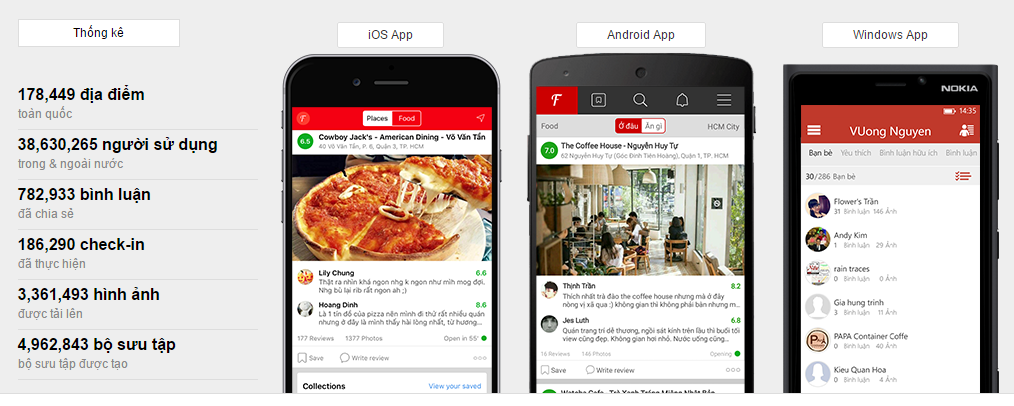
\includegraphics[width=\linewidth]{foody}
				\caption{Giao diện và các thống kê về trang \textit{foody.vn}}
				\label{fig:foody}
			\end{figure}

			\par Như đã trình bày ở phần 2.1, MXH nói chung có thể biểu diễn bằng đồ thị với nốt là các tác nhân và cạnh đại diện cho mối quan hệ hoặc tương tác giữa các nốt đó. Đối với MXH \textit{Foody} , mỗi nốt là người dùng hoặc địa điểm, mỗi cạnh giữa một nốt là người dùng và một nốt là địa điểm được thể hiện qua review của người dùng cho địa điểm hoặc comment trên các review. Ngoài ra giữa các nốt là người dùng còn tồn tại các cạnh là quan hệ “theo dõi” giữa họ. Trong đó, mối quan hệ được xét đến chủ yếu trong phạm vi đề tài là \textit{review} của người dùng đối với địa điểm.


			% Vẽ mô hình mạng foody
			\begin{figure}[h!]
				\begin{tikzpicture}[x=1.5cm, y=1.5cm, >=stealth]

\foreach \m/\l [count=\y] in {1,2,3,missing,4}
  \node [every neuron/.try, neuron \m/.try] (input-\m) at (1,2.5-\y) {};

\foreach \m [count=\y] in {1,2,3,missing,4}
  \node [every neuron/.try, neuron \m/.try ] (hidden-\m) at (3,2.5-\y) {};

\foreach \l [count=\i] in {1,2,3,n}
	\node [left=0.5cm] at (input-\i.west)  {Người dùng \l};

\foreach \l [count=\i] in {1,2,3,n}
	\node [right = 0.5cm] at (hidden-\i.east)  {Địa điểm \l};

% Tạo các đường liên kết
\foreach \i in {1,2}
  \foreach \j in {1}
    \draw [->] (input-\i) -- (hidden-\j);

\foreach \i in {1,2,4}
  \foreach \j in {2}
    \draw [->] (input-\i) -- (hidden-\j);

\foreach \i in {3}
  \foreach \j in {3}
    \draw [->] (input-\i) -- (hidden-\j);

\foreach \i in {3,4}
  \foreach \j in {4}
    \draw [->] (input-\i) -- (hidden-\j);


% Tạo chú thích bên cạnh
\foreach \m/\l [count=\y] in {1}
  \node [every neuron/.try, neuron \m/.try] (user-\m) at (7,2.5-\y*3) {};

\foreach \m/\l [count=\y] in {1}
  \node [every neuron/.try, neuron \m/.try] (res-\m) at (9,2.5-\y*3) {};

\foreach \l [count=\i] in {1}
  \node [above] at (user-\i.north) {Người dùng i};

\foreach \l [count=\i] in {1}
  \node [above] at (res-\i.north) {Địa điểm j};

\foreach \i in {1}
  \foreach \j in {1}
    \draw [->] (user-\i) -- (res-\j)
	node [above, midway] {(i,j)}
	node [below=0.8cm, midway] {\textit{Review của người dùng i về địa điểm j}};


\end{tikzpicture}
				\caption{Mô hình hóa mạng xã hội \textit{foody.vn}}
				\label{fig:foodygraph}
			\end{figure}

			\par Người chủ địa điểm ăn uống có thể vào trang mạng \textit{foody.vn} xem các review và rating của người dùng đối với địa điểm của mình, từ đó đánh giá được độ thu hút của địa điểm ở hiện tại. Sẽ là hữu ích nếu có một hệ thống dự đoán trước được số lượng các review và điểm rating đối với địa điểm của họ trong tương lai. Những thông tin này sẽ là căn cứ để người chủ địa điểm xem xét mức độ thu hút của địa điểm trong tương lai và có thể đưa ra giải pháp cải thiện. Đề tài được sinh ra là để hướng tới những người chủ địa điểm đó.

			\par Dữ liệu trên trang \textit{Foody}  với các nốt và liên kết đã được giải thích ở trên là cơ sở để thực hiện các phân tích trên nó, nhằm tạo ra một hệ thống học máy giải quyết vấn đề đưa ra. Vấn đề này có thể coi là một dạng của Dự đoán liên kết, ở đó mục tiêu là dự đoán xem trong tương lai sẽ có thêm bao nhiêu review nữa, tức là bao nhiêu cạnh nữa giữa các người dùng và một địa điểm sẽ được hình thành. Đồng thời một mục tiêu khác của bài toán là dự đoán một đặc điểm của nốt trong tương lai, đó là số điểm rating trung bình của một địa điểm. Để đạt được những mục tiêu vừa nêu, cần có thêm những kiến thức về Khai phá dữ liệu dạng văn bản và Phân loại nốt. Những sự liên hệ này sẽ được dẫn ra rõ hơn ở những phần tiếp theo.

			\begin{figure}[h!]

% Vẽ vấn đề
\begin{tikzpicture}[square/.style={rectangle, draw}]
        \node at (0,0) [square,draw, text width = 4cm] (c100) {Thông tin liên quan đến địa điểm A cho tới thời điểm hiện tại
};
        \node at (5.5,0) [square,draw, text width = 5cm, align = center] (v100) {\textbf{HỆ THỐNG}};
	\node at (11.5,0) [square,draw, text width = 5cm] (d100) { 
		\begin{itemize}
        \item Số review của A ở mốc thời gian t trong tương lai.
        \item Điểm rating trung bình của A ở mốc thời gian t trong tương lai.
   	 \end{itemize}};
        \draw [->](c100) -- (v100);
	 \draw [->](v100) -- (d100);
    \end{tikzpicture}
				\caption{Mô hình hóa bài toán đề xuất}
				\label{fig:problem}
			\end{figure} 

		\subsection{Các nghiên cứu liên quan}
			\par Yelp là một trang MXH về địa điểm nổi tiếng ở Mỹ với những chức năng tương tự như trang MXH \textit{Foody}  của Việt Nam. Trang MXH này tổ chức ra một cuộc thi mang tên Yelp Dataset Challenge (bắt đầu từ năm 2014, đến nay đã trải qua 6 vòng thi và đang ở vòng 7), thu hút hàng trăm bài nghiên cứu của các tác giả khắp thế giới. Nhiều bài toán được đưa ra dựa trên tập dữ liệu do cuộc thi này cung cấp, \textit{ví dụ}: gợi ý các địa điểm phù hợp với sở thích, thói quen của người dùng [4], [5]; tóm tắt, trực quan hóa review cho người dùng [6] hay dự đoán tương lai của địa điểm ăn uống.
			\par Trong đó, nhóm bài toán có nhiều mối liên hệ nhất với đề tài do nhóm đề xuất là những bài toán về Dự đoán tương lai của một địa điểm ăn uống:
			\begin{itemize}
				\item Trong [7], tác giả đã đề xuất ra mô hình học máy nhằm dự đoán xem liệu một địa điểm sẽ tiếp tục hoạt động hay đóng cửa. Đó là một bài toán phân loại nhị phân với đầu vào là các thông tin liên quan tới địa điểm và đầu ra là một trong hai nhãn cho địa điểm: “open” – Địa điểm tiếp tục hoạt động, hoặc “close” – Địa điểm sẽ bị đóng cửa. Tác giả dùng 4 nhóm thuộc tính khác nhau cho mô hình học máy:
					\begin{itemize}
						\item Nhóm các thuộc tính liên quan đến đánh giá: Số lượng review tương ứng, điểm rating trung bình, số lượng người dùng checkin.
						\item Nhóm các thuộc tính về vị trí địa lý: Kinh độ, vĩ độ, bang.
						\item Nhóm các thuộc tính liên quan thời gian: Thời gian (ngày) từ bài review cuối tới hiện tại, thời gian (ngày) từ bài tip cuối cùng tới hiện tại.
						\item Nhóm thuộc tính liên quan đến dữ liệu văn bản trong review.
					\end{itemize}
					Kết quả chỉ ra rằng nhóm thuộc tính về vị trí địa lý và nhóm liên quan đến thời gian cho hiệu quả dự đoán cao nhất.
				\item Trong [8], tác giả đã đề xuất một tập các thuộc tính dựa trên đặc trưng của địa điểm cũng như dữ liệu văn bản trên review đối với địa điểm đó và dùng các mô hình học máy khác nhau (Logistic Regression, Support Vector Machine, Tree and Random Forest Classifier, Support Vector Regression) để dự đoán điểm rating cho địa điểm. Bài toán dự đoán điểm rating cho địa điểm được quy về bài toán phân loại cho địa điểm với các nhãn là 0,1,2,3,4,5 chính là điểm rating (được làm tròn) cho địa điểm đó. Kết quả cuối cùng cho thấy các thuộc tính liên quan đến phân tích ý kiến trên review, số lượng review, vị trí của địa điểm và số lượng các địa điểm nằm ở khu vực lân cận là những thuộc tính quan trọng nhất.
				\item Điểm rating đối với một địa điểm là cơ sở quan trọng để một người dùng đưa ra lựa chọn có tới địa điểm đó hay không. Nhưng đôi khi việc rating của người dùng cũng mang tính chất chủ quan và thiên vị. \textit{Ví dụ:} Trên Yelp, người A đánh giá nhà hàng D ăn ngon, phục vụ tốt nhưng cho điểm là 4, trong khi người B có những đánh giá tương tự cho D nhưng cho điểm tới 5. Do đó một ý tưởng được đưa ra là dự đoán rating cho một địa điểm chỉ dựa trên dữ liệu văn bản trong review đối với địa điểm. Trong [9], tác giả tạo một nhóm gồm các từ thông dụng thường xuất hiện nhất trong các bài review và dùng các từ trong nhóm này để tạo tập thuộc tính phục vụ cho hệ thống dự đoán rating. Các mô hình học máy được sử dụng là: Linear Regression, Support Vector Regression, Support Vector Regression với tập thuộc tính được chuẩn hóa và Decision Tree Regression.
				\item Trong [10], một mô hình học máy dựa trên Support Vector Regression được đề xuất nhằm dự đoán mức độ thu hút của một địa điểm trong tương lai. Mức độ thu hút này được đánh giá theo thước đo là số lượng review đối với địa điểm trong tương lai (số lượng review mà địa điểm nhận được trong 6 tháng tới). Mô hình này dựa trên hai nhóm thuộc tính chính: Nhóm thuộc tính được lấy ra từ tập dữ liệu của Yelp như điểm rating, vị trí của địa điểm, thời gian (ngày) từ bài review gần nhất… và nhóm thuộc tính được trích xuất từ review của địa điểm (Khai phá dữ liệu dạng văn bản). Các nhóm thuộc tính này là cơ sở cho việc đề xuất tập thuộc tính của nhóm.
				\item Trong [11], tác giả đề xuất ra hai mô hình dự đoán mức độ thu hút của một địa điểm trong tương lai, một mô hình dựa trên mô hình Chuỗi thời gian (Time Series) và một mô hình khác dựa trên Dự đoán liên kết trong đồ thị hai phía (Bipartite Graph). Mức độ thu hút này được thể hiện qua số lượng review mà địa điểm nhận được trong tương lai và số điểm rating tại thời điểm đó. Hai mô hình này sử dụng tập thuộc tính tương tự như trong [10] nhưng không có nhóm thuộc tính liên quan tới dữ liệu văn bản trong các review. Một trong số các mô hình được nhóm đề xuất thực hiện cũng được đưa ra dựa trên ý tưởng của mô hình theo Chuỗi thời gian được nói tới trong bài. 
				\item Trong [12], tác giả cũng đưa ra bài toán dự đoán xu hướng của địa điểm dựa vào số lượng review nhận được trong tương lai (Số lượng review nhận được trong tháng tới) sử dụng các phân tích thống kê trên mô hình Chuỗi thời gian.
			\end{itemize}
			\par Ở Việt Nam, từ dữ liệu của trang mạng \textit{Foody}  và các trang mạng xã hội về địa điểm khác, một số đề tài cũng đã được thực hiện:
			\begin{itemize}
				\item Trong [13] và [14], tác giả đã đưa ra bài toán Đề xuất địa điểm dựa trên dữ liệu của mạng \textit{Foody}  và dẫn ra những phương pháp cơ bản để giải quyết bài toán này, đó là phương pháp Lọc – Cộng tác (Collaborative Filtering), lọc dựa trên nội dung (Content-based Filtering) và phương pháp lai (Hybrid) như là sự kết hợp giữa hai phương pháp trên. Dữ liệu dùng cho phân tích được crawl từ trang \textit{foody.vn}, giải thuật học máy sẽ học những đặc trưng của địa điểm, hồ sơ của người dùng, và kết hợp với dữ liệu về mặt địa lý để hạn chế các kết quả không hợp lý về mặt khoảng cách. 
				\item Trong [15], tác giả sử dụng các kỹ thuật Khai phá dữ liệu dạng văn bản (Trên tiếng Việt) để phân tích các bình luận và review của người dùng đối với các địa điểm trên \textit{foody.vn} và \textit{diadiemanuong.com}. Các câu trong các bình luận và review này được chia thành 5 chủ đề: giá cả, khu vực, dịch vụ, không gian và chất lượng. Sau đó, phân tích các từ trong mỗi câu để chỉ ra ý kiến của người dùng đối với địa điểm là tích cực hay tiêu cực. Kết quả cuối cùng sẽ có được bằng cách tính trung bình xem bao nhiêu phần trăm đánh giá là tích cực hay tiêu cực đối với địa điểm, và ứng với từng chủ đề trong số 5 chủ đề trên.   
				\end{itemize}
			\par Những thành công nhất định trong các nghiên cứu trên là cơ sở quan trọng để nhóm đưa ra đề xuất cho phương pháp giải quyết thực hiện đề tài.


\section{Kiến thức nền tảng}
		\subsection{Tối ưu tập thuộc tính}
			\par Việc tối ưu tập thuộc tính là xác định các thuộc tính quan trọng và loại bỏ các thuộc tính dư thừa, nhiễu để làm giảm số chiều của không  gian thuộc tính, qua đó cải thiện độ chính xác và tốc độ tính toán của hệ thống. Các giải thuật để tối ưu tập thuộc tính liên quan đến đề tài gồm: Principal Components Analysis, Univariate Feature Analysis và Recursive Feature Elimination.
			\par \textbf{Principal Components Analysis (PCA)}
				\par \textit{Định nghĩa} 
				\par PCA là một thuật toán thống kê sử dụng phép biến đổi trực giao để biến đổi một tập hợp dữ liệu từ một không gian nhiều chiều sang một không gian mới ít chiều hơn (2 hoặc 3 chiều) nhằm tối ưu hóa việc thể hiện sự biến thiên của dữ liệu. 
				\par  \textit{Ý tưởng}
				\par Tìm ra một không gian mới với số chiều nhỏ hơn không gian cũ với tiêu chí cố gắng phản ánh được càng nhiều thông tin gốc càng tốt, và thước đo cho khái niệm “thông tin” ở đây là phương sai. Đồng nghĩa với việc tìm những thuộc tính mới từ tổ hợp tuyến tính các thuộc tính cũ sao cho mỗi thuộc tính mới có phương sai càng lớn càng tốt. 
				\par  \textit{Kiến thức cơ bản}
				\par Độ lệch chuẩn (Standard Deviation), Phương sai (Variance), Hiệp phương sai (Covariance), Ma trận hiệp phương sai (The covariance matrix), Eigenvectors, Eigenvalues [16]. 
				\par \textit{Phương pháp}
				\par Để xác định các chiều của không gian mới, ta lần lượt thực hiện 3 bước tổng quát:
				\begin{enumerate}
					\item Xử lý dữ liệu:
					\par Cho ma trận ${X= \big\{ x_{ij} \big\}  \in  \mathbb{R}^{n \times p}}$, trong đó \textit{n} là số mẫu, \textit{p} là số thuộc tính.
					\par Mỗi thuộc tính có một giá trị trung bình cộng:
					\begin{center}
						\par ${\overline{x}_{j}=\frac{\sum_{i=1}^n{x_{ij}}}{n}}$
					\end{center}
					\par Chuẩn hóa dữ liệu ta được ma trận mới ${X^{new}=\left\{x_{ij}^{new}\right\}}$, trong đó:
					\begin{center}
						\par ${x_{ij}^{new}=x_{ij}-\overline{x}_{j}}$
					\end{center}
					\item Tính ma trận hiệp phương sai của ma trận đã chuẩn hóa.
					\item Tính các eigenvector, eigenvalue của ma trận hiệp phương sai. Mỗi eigenvector đại diện cho một thuộc tính, eigenvalue tương ứng càng lớn thì thuộc tính đó càng quan trọng.
				\end{enumerate}
				\par Thuật toán chi tiết và các ví dụ dễ hiểu kèm theo được trình bày ở [16].
				\par  \textit{Ưu điểm}
				\begin{itemize}
					\item{Phương pháp học không giám sát, do đó PCA sẽ tự động tìm ra được các thuộc tính đặc trưng mà con người không nhận ra được.}
					\item{Làm giảm độ nhiễu của tập dữ liệu.}
				\end{itemize}
				\par  \textit{Nhược điểm}
				\begin{itemize}
					\item{PCA chỉ làm việc với dữ liệu số.}
					\item{PCA phù hợp sử dụng đối với tập dữ liệu tuyến tính, do đó khi dữ liệu là phi tuyến thì dùng PCA thôi là chưa đủ.}
					\item{Quy tắc phương sai lớn nhất thì thuộc tính quan trọng nhất không luôn luôn đúng.}
				\end{itemize}
			\par \textbf{Univariate Feature Analysis}
				\par \textit{Định nghĩa} 
				\par Univariate Feature Analysis là giải thuật xác định thuộc tính quan trọng dựa trên ý tưởng theo dõi ảnh hưởng của mỗi thuộc tính một cách độc lập đến hiệu suất dự đoán của hệ thống rồi sau đó chọn ra $n$ thuộc tính mang lại hiệu suất tốt nhất làm tập thuộc tính cho mô hình học máy [17].
				\par \textit{Phương pháp}
				\begin{enumerate}
					\item Lựa chọn một thuộc tính bất kỳ, xây dựng hệ thống dựa chỉ dựa trên thuộc tính đó, đánh giá hệ thống: đối với bài toán hồi quy sử dụng giá trị \textit{f-regression}.
					\item Lựa chọn n thuộc tính có giá trị \textit{f-regression} lớn nhất.
				\end{enumerate}
				\par  \textit{Ưu điểm}
				\par Giải thuật đơn giản và thời gian chạy nhanh.
				\par  \textit{Nhược điểm}
				\par Những thuộc tính tốt nhất mà thuật toán chọn ra đều ảnh hưởng độc lập đến kết quả bài toán. Tuy nhiên, đôi khi việc kết hợp các thuộc tính không tốt với nhau cũng có thể đưa ra mô hình dự đoán tốt.
			\par \textbf{Recursive Feature Elimination}
				\par \textit{Định nghĩa} 
				\par Recursive Feature Elimination là giải thuật xác định thuộc tính quan trọng dựa trên ý tưởng áp dụng giải thuật trên tất cả các thuộc tính, sau đó loại bớt các thuộc tính sao cho giải thuật đạt kết quả tối ưu nhất [17].
				\par \textit{Phương pháp}
				\begin{enumerate}
					\item Train giải thuật trên tập các thuộc tính và sau đó gán trọng số (\textit{Ví dụ}: hệ số của mô hình tuyến tính) cho mỗi thuộc tính.
					\item Thuộc tính có trị tuyệt đối của trọng số tương ứng nhỏ nhất sẽ bị loại khỏi tập thuộc tính. Sau đó lặp lại bước 1. Quá trình lặp kết thúc khi giải thuật đạt được hiệu suất mong muốn hoặc đã đạt đến số thuộc tính mong muốn.

				\end{enumerate}
				\par  \textit{Ưu điểm}
				\par Kết quả thu được tốt hơn khi phân tích ảnh hưởng của thuộc tính đến kết quả một cách độc lập.
				\par  \textit{Nhược điểm}
				\par Chi phí tính toán cao.		
		\subsection{Gán nhãn cụm từ trong Xử lý ngôn ngữ tự nhiên}
			\par Trong Xử lý ngôn ngữ tự nhiên, để thực hiện được quá trình phân tích cú pháp thì một trong những vấn đề quan trọng là gán nhãn cho các từ/cụm từ ở trong văn bản, tức là “bẻ” các câu trong văn bản đó ra thành những thành phần nhỏ hơn (từ và cụm từ) sau đó xác định từ loại tương ứng với mỗi từ và cụm từ đó [18]. Bảng 1 minh họa quá trình phân tích cú pháp câu "\textit{Món lẩu ở nhà hàng đó rất ngon}".
			\begin{table}[h]
				\centering
				\caption{Ví dụ xác định từ loại tương ứng mỗi từ và cụm từ}
				\label{my-label}
				\begin{tabular}{|c|c|c|c|c|c|c|}
				\hline
           				Món &   lẩu        &  ở &  nhà hàng          &  đó          &       rất     & ngon           \\ \hline
          					N & N          & P  &    N       &       ART    &     ADV      &     ADJ      \\ \hline
				\multicolumn{2}{|c|}{NP} &  & \multicolumn{2}{c|}{NP} &  \multicolumn{2}{c|}{VP} \\ \hline
				\multicolumn{2}{|c|}{} & \multicolumn{3}{c|}{PP}    &           &           \\ \hline
				\multicolumn{5}{|c|}{NP}                          &           &           \\ \hline
				\end{tabular}
			\end{table}
			\par Trong đó, \textit{N}: Danh từ,  \textit{P}: Giới từ,  \textit{ART}: Mạo từ,  \textit{ADV}: Trạng từ,  \textit{NP}: Cụm danh từ,  \textit{PP}: Cụm giới từ.
		\subsection{Chuỗi thời gian (Time Series)}
			\par Chuỗi thời gian là một chuỗi các điểm dữ liệu, được đo theo từng khoảng thời gian bằng nhau. \textit{Ví dụ:} theo từng tháng, từng năm. Công thức chuỗi thời gian [19]:
			\begin{center}
				$y_{t}=f(y_{t-1},y_{t-2},...,y_{t-n}) + w(t)$
			\end{center}
			\par Từ công thức, ta nhận thấy có thể dự đoán sự kiện thời gian tại $t$ ($y_{t}$) dựa vào các sự kiện đã biết trong quá khứ ($y_{t-1},y_{t-2},...,y_{t-n}$); $w(t)$: thông tin chưa biết tạo nên độ nhiễu. Vấn đề dự đoán dựa trên Chuỗi thời gian có thể xem là giải bài toán Hồi quy cơ bản có giám sát (Generic Supervised Learning Regression). \textit{Ví dụ}: Bài toán dự đoán doanh số bán sản phẩm của quí (năm) tới dựa vào doanh số bán của các quí (năm) qua.
		\subsection{Giải thuật học máy Support Vector Regression}
			\par Trong lĩnh vực học máy, Support Vector Regression (SVR) là mô hình học có giám sát, được sử dụng vào bài toán phân tích hồi quy. Mô hình SVR là một mở rộng của giải thuật Support Vector Machine (SVM).
			\par \textbf{Ý tưởng}
				\par Giả sử có tập dữ liệu gồm $l$ mẫu $\left\{\left(x_{1},y_{1}\right),\left(x_{2},y_{2}\right),...,\left(x_{l},y_{l}\right)\right\}$, với $x_{i}\in  \mathbb{R}^{n}$ và $y_{i}\in  \mathbb{R}$ với mọi i. Mục đích của mô hình SVR là đi tìm một hàm \textit{f(x)} sao cho số lượng các mẫu $\left(x_{i},y_{i}\right)$ thỏa mãn điều kiện $\mid y_{i} - f(x_{i})\mid \leq \epsilon $ ($\epsilon$ cho trước) là lớn nhất [20]. Hình 4 mô tả ý tưởng giải thuật: Hàm $f(x)$ sẽ tạo ra một đường thẳng (siêu phẳng đối với không gian nhiều chiều), kết hợp giá trị $\epsilon$ tạo nên hai đường biên kèm theo (hai đường nét đứt); bài toán là tìm hàm $f(x)$ sao cho mọi điểm trong tập mẫu đều nằm trong vùng giữa hai đường biên tạo ra.
				\begin{figure}[h!]
				\begin{center}
%vẽ ý tưởng SVR
\begin{tikzpicture}[]
  % Draw axes
 \draw[thick,->] (0,0) -- (6.5,0) node[anchor=north west] {x axis};
\draw[thick,->] (0,0) -- (0,7.5) node[anchor=south east] {y axis};
  % draw line
  \draw (0,-1) -- (6,5); % y=x-1
  \draw[dashed] (-1,0) -- (6,7); % y=x+1
  \draw[dashed] (2,-1) -- (6,3); % y=x-3
  % \draw labels
  \draw (3.5,3) node[rotate=45,font=\small] 
        {$ f(x) = \mathbf{w}\cdot \mathbf{x} + b $};
  % draw negative dots
  \fill[black] (1,1.5)     circle (3pt);
  \fill[black] (2.75,1.25)    circle (3pt);
  \fill[black] (-0.6,-0.5)   circle (3pt);
  \fill[black] (2, -0.4) circle (3pt);
  \fill[black] (4,4)     circle (3pt);
  \fill[black] (4.5,1.5)   circle (3pt);
  \fill[black] (5,6)   circle (3pt);
\fill[black] (6.1,7) rectangle (6.3,7.01);
\draw (6.7,7) node {\large{$+ \epsilon$}}; 
\fill[black] (6.1,3) rectangle (6.3,3.01);
\draw (6.7,3) node {\large{$- \epsilon$}}; 
\fill[black] (6.1,5) rectangle (6.3,5.01);
\draw (6.7,5) node {\large{$0$}};
\draw[thick] (6.2,7) -- (6.2,3);
\end{tikzpicture}
				\end{center}
					\caption{Minh họa mô hình SVR}
				\label{fig:foody}
			\end{figure}
				\par Trường hợp hàm f(x) tuyến tính, biểu diễn dạng:
					\begin{center}
						$f(x)=\langle w,x\rangle + b \;với \;w\in \mathbb{R}^{n}, b\in \mathbb{R}$
						\par $\langle .,.\rangle$ : Tích có hướng của hai vector
					\end{center}
				\par Hàm f(x) càng tối ưu khi chuẩn của vector w càng nhỏ. Khi đó bài toán đặt ra là:
					\begin{center}
						$minimize \: \frac{1}{2}\parallel{w}\parallel^{2}$ \\
						$subject\; to \: \begin{cases}y_{i}-\langle w,x_{i}\rangle-b \leq \epsilon \\\langle w,x_{i}\rangle-b-y_{i} \leq \epsilon\end{cases}$
					\end{center}
				\par Giả thuyết bài toán như trên có nghĩa là ta có thể tìm hàm $f(x)$ thỏa mãn điều kiện: mọi điểm $(x_{i},y_{i})$ đều nằm trong vùng của hai đường biên được tạo ra quanh đường thằng tạo bởi f(x). Tuy nhiên, trên thực tế có những trường hợp mà không thể tìm hàm $f(x)$ thỏa mãn điều kiện đó, hoặc ta muốn tạo một ít sai số cho mô hình để tránh trường hợp overfitting. Do vậy, ta phải thay đổi yêu cầu để luôn tìm ra hàm $f(x)$. Ý tưởng là hàm f(x) vẫn được chấp nhận khi tồn tại một số điểm $(x_{i},y_{i})$ không nằm trong vùng giữa hai đường biên. Những điểm $(x_{i},y_{i})$ tạo nên sai số của hàm $f(x)$, kí hiệu tổng sai số đó là E. Yêu cầu bài toán bây giờ là tìm $min \parallel w\parallel$ và $min(E)$. Với ý tưởng đó, bài toán được mô hình hóa lại:
					\begin{center}
						$minimize \: \frac{1}{2}\parallel{w}\parallel^{2} +C\sum_{i=1}^l(\xi_{i}+\xi_i^*)$ \\
						$subject\; to \: \begin{cases}y_{i}-\langle w,x_{i}\rangle-b \leq \epsilon + \xi_{i}\\\langle w,x_{i}\rangle-b-y_{i} \leq \epsilon+\xi_i^* \\ \xi_{i},\xi_i^* \geq0\end{cases}$
					\end{center}
				\par Trong đó:
				\begin{itemize}
					\item $\xi_{i}, \xi_i^*$ : Trường hợp điểm $(x_{i},y_{i})$ nằm trong vùng hai đường biên, hai giá trị này đều bằng 0. Trường hợp $(x_{i},y_{i})$ nằm ngoài hai vùng hai đường biên tạo ra thì một trong hai giá trị sẽ là $\mid y_{i} - f(x_{i})-\epsilon\mid$ và giá trị còn lại bằng 0. Bản chất  $\xi_{i} + \xi_i^ * = \xi= \mid y_{i} - f(x_{i})-\epsilon\mid$, sử dụng hai biến thay vì một biến $\xi$ nhằm mục đích loại bỏ dấu giá trị tuyệt đối, đơn giản trong việc tính toán sau này.
					\item $\sum_{i=1}^l(\xi_{i}+\xi_i^*)$ : Tổng sai số của hàm $f(x)$. Hàm sai số là hàm Vapnik's $\epsilon - insensitive$: Mỗi mẫu $(x_{i},y_{i})$ nếu nằm trong vùng hai đường biên thì không gây ra lỗi, những điểm nằm ngoài sẽ gây nên lỗi là $\mid y_{i} - f(x_{i})-\epsilon\mid$. Công thức hàm Vapnik's $\epsilon - insensitive$:
					\begin{center}
						$\mid y_{i} - f(x_{i})\mid_{\epsilon} \:=\:\begin{cases}0 &  if \mid y_{i} - f(x_{i})\mid \:\leq \epsilon\\\mid y_{i} - f(x_{i})\mid - \: \epsilon & otherwise\end{cases} $ 
					\end{center}
					\item $C$ : Giá trị điều chỉnh giữa việc tối thiểu chuẩn vector $w$ và tổng giá trị sai số. Nếu C quá lớn thì thuật toán thiên về mục đích là điều chỉnh sao cho tổng giá trị sai số là nhỏ nhất, và ngược lại.
				\end{itemize}
			\par Hình 5 mô tả ý tưởng giải thuật SVR, tồn tại các điểm nằm ngoài vùng hai đường biên và đồng thời  chỉ có các điểm đó mới gây nên sai số theo công thức hàm  Vapnik's $\epsilon - insensitive$.
			\par Ý tưởng tiếp theo quan trọng là sử dụng hàm Lagrange (Lagrange function) từ mục tiêu bài toán và các ràng buộc để tìm ra các giá trị w, b.
				\begin{figure}[h!]
				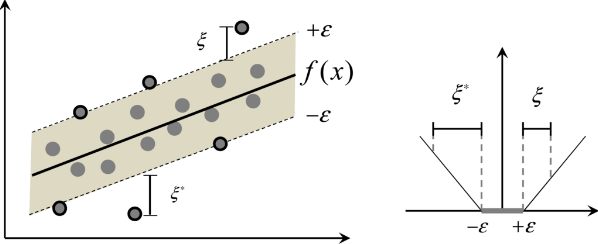
\includegraphics[width=\linewidth]{svr}
				\caption[Minh họa cách tính sai số trong mô hình SVR]{Ý tưởng giải thuật SVR gắn liền với hàm sai số Vapnik's $\epsilon - insensitive$  
					(\textit{Tham khảo:} Kang Yu, Georg Leufen (2013) Investigation of Leaf Diseases and Estimation of Chlorophyll Concentration in Seven Barley Varieties Using Fluorescence and Hyperspectral Indices)}
				\label{fig:svr}
			\end{figure}
				
			\par \textbf{Kĩ thuật Kernel}
			\par Trong nhiều trường hợp, ta không thể tìm được siêu phẳng (hàm \textit{f(x)}) thỏa mãn yêu cầu nằm gần với tất cả các điểm dữ liệu. Khi đó, chúng ta sử dụng kĩ thuật ánh xạ không gian hiện tại sang không gian nhiều chiều hơn, ở đó ta có thể tìm ra siêu phẳng thỏa mãn. Sử dụng hàm $(\phi(x))$ biến đổi vector $x$ hiện tại sang không gian nhiều chiều hơn. Lúc đó hàm $f(x)$ có dạng là: $f(x)=\langle w,\phi(x)\rangle + b$. Hình 6 minh họa lý thuyết Kernel: Ở không gian ban đầu (bên trái), ta không thể tìm được siêu phẳng; sau khi chuyển sang không gian mới (bên phải) nhờ hàm $\phi(x)$ thì tìm được siêu phẳng mong muốn.
				\begin{figure}[h!]
				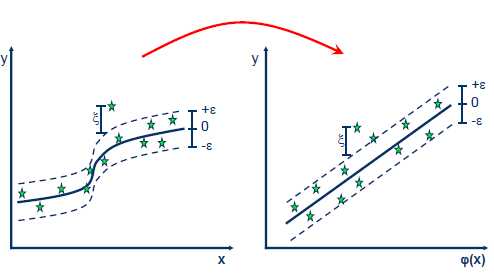
\includegraphics[width=\linewidth]{kernel}
				\caption[Ý tưởng kĩ thuật Kernel]{Ý tưởng kĩ thuật Kernel (\textit{Tham khảo:} Dr. Saed Sayad, Support Vector Machine - Regression (SVR))}
				\label{fig:svr}
			\end{figure}
	\section{Phương pháp đề xuất}								
		\subsection{Tập dữ liệu}
			\par \textit{foody.vn} là trang web chứa thông tin về các địa điểm ăn uống ở Việt Nam (đặc biệt là TP. Hồ Chí Minh) với lượng thông tin phong phú và đáng tin cậy. Dữ liệu được dùng cho việc phân tích được crawl từ trang web \textit{foody.vn} dùng thư viện jsoup và crawljax trên ngôn ngữ Java và được lưu trong một cơ sở dữ liệu không quan hệ (MongoDb). Jsoup và crawljax đều là các thư viện mã nguồn mở trên Java hỗ trợ việc trích xuất thông tin từ các trang web với API đơn giản và dễ sử dụng.
			\par \textbf{Dữ liệu về địa điểm:}\\
				"type": "business"\\
				"businessId": (business\_id)\\
				"name": (business\_name)\\
				"priceRange":(lowestPrice - highestPrice)\\
				"aggregateRating":\\
				\hspace*{1.5cm}"ratingValue": (avarage\_rating)\\
				\hspace*{1.5cm}"reviewCount": (review\_count)\\
				\hspace*{1.5cm}"bestRating": (best\_rating)\\
				\hspace*{1.5cm}"worstRating": (worst\_rating)\\
				"open": (open\_hours)\\
				"address": \\
				\hspace*{1.5cm}"addressLocality": (district\_name)\\
				\hspace*{1.5cm}"addressRegion": (province\_name)\\
				\hspace*{1.5cm}"streetAddress": (street\_name)\\
				"geo":\\
				\hspace*{1.5cm}"latitude": (latitude)\\
				\hspace*{1.5cm}"longitude": (longitude)\\

			\par \textbf{Dữ liệu về người dùng:}\\
				"type": "user"\\
				"userId": (user\_id)\\
				"name": (user\_name)\\
				"birthdate": (birth\_date)\\
				"gender": (nam\_nu)\\
				"maritalStatus": (docthan\_dakethon)\\
				"address": (address\_string)\\
				"reviewCount": (num\_of\_reviews\_create)\\

			\par \textbf{Dữ liệu về review:}\\
				"type": "review"\\
				"reviewId": (review\_id)\\
				"userId": (user\_id)\\
				"businessId": (business\_id)\\
				"content": (content\_text)\\
				"date": (date\_created)\\
				"rating":\\
				\hspace*{1.5cm}"space": (space\_rating)\\
				\hspace*{1.5cm}"position": (position\_rating)\\
				\hspace*{1.5cm}"quality": (quality\_rating)\\
				\hspace*{1.5cm}"reservation": (reservation\_rating)\\
				\hspace*{1.5cm}"price": (price\_rating)\\		
				"likes": [array\_of\_userId]
					
		\subsection{Tập thuộc tính}
			\par Nhóm đề xuất 4 nhóm thuộc tính: nhóm thuộc tính của địa điểm ăn uống trong một khoảng thời gian bất kì, nhóm thuộc tính của địa điểm ăn uống trong một khoảng thời gian từ lúc thành lập đến hiện tại, nhóm thuộc tính trích xuất ra từ các review đối với địa điểm, và nhóm thuộc tính dựa trên phân loại người dùng. 
			\par \textbf{Thuộc tính phụ thuộc khoảng thời gian bất kì (5.2.1)}
				\par Kí hiệu địa điểm ăn uống là M. Khoảng thời gian (t1,t2) có thời điểm bắt đầu là t1 và thời điểm kết thúc là t2. Khi đó tập thuộc tính đặc trưng cho khoảng thời gian (t1,t2) là:
				\begin{enumerate}
					\item Số lượng review M nhận được trong khoảng thời gian (t1,t2).
					\item Số điểm trung bình M nhận được trong khoảng thời gian (t1,t2).
					\item Số lượng review M nhận được được yêu thích trong khoảng thời gian (t1,t2).
					\item Số điểm cao nhất M nhận được: tính từ khi địa điểm hình thành đến hiện tại.	
					\item Số điểm thấp nhất M nhận được: tính từ khi địa điểm hình thành đến hiện tại.
					\item Số ngày giữa bài review đầu tiên M nhận được đến t2.
					\item Số ngày giữa bài review cuối cùng M nhận được đến t2.
					\item Số ngày giữa bài review đầu tiên của địa điểm đến bài review cuối cùng địa điểm nhận được tính tới t2.
				\end{enumerate}
			\par \textbf{Thuộc tính phụ thuộc thời gian (5.2.2)}
				\par Tập hợp thuộc tính đặc trưng cho địa điểm ăn uống M, tính từ khi M thành lập đến hiện tại:
				\begin{enumerate}
					\item Số bài review M nhận được.
					\item Số điểm cao nhất M nhận được.
					\item Số điểm thấp nhất M nhận được.
					\item Số điểm trung bình M nhận được.
					\item Số địa điểm ăn uống cùng loại với M.
					\item Số địa điểm ăn uống trong bán kính 1km của M.
					\item Số bài review về M được yêu thích.
					\item Số ngày kể từ bài review cuối cùng về M. 
					\item Số ngày kể từ bài review đầu tiên về M.
					\item Số ngày giữa bài review đầu tiên và cuối cùng về M. 
					\item Số lượng bài review cao nhất trong 1 ngày M nhận được.
					\item Số ngày kể từ bài review cuối cùng về một địa điểm ăn uống cùng loại với M.
					\item Số lượng bài review của tất cả nhà hàng cùng loại với M.
					\item Số lượng bài review của tất cả nhà hàng trong bán kính 1km của M.	
					\item Số lượng bài review được yêu thích của tất cả địa điểm ăn uống cùng loại với M.
					\item Số lượng bài review được yêu thích của tất cả địa điểm ăn uống trong bán kính 1km của M.
					\item Số ngày kể từ bài review cuối cùng về bất kỳ một địa điểm ăn uống trong bán kính 1km.
				\end{enumerate}
			\par \textbf{Thuộc tính trích xuất từ review (5.2.3)}
				\par Mục tiêu của nhóm là tìm ra K từ/cụm từ (khoảng 100)phổ biến nhất (keyword) trong tất cả các bài review trên \textit{foody.vn} và  xem chúng là tập thuộc tính của một bài review. Sau đó với mỗi bài review, ta xem mỗi thuộc tính có bao nhiêu lần được đánh giá tích cực, bao nhiêu lần được đánh giá tiêu cực. Dữ liệu được dùng cho việc trích xuất này là mọi review của mọi địa điểm có trong tập dữ liệu. Thực hiện thứ tự các bước:
			 	\begin{enumerate}
					\item \textit{Tiền xử lý cho các review}
						\par Như đã trình bày ở phần 3.3, dữ liệu dạng văn bản trên MXH có đặc trưng là Ngắn gọn và Phi cấu trúc, do đó cần có quá trình tiền xử lý để giải quyết những điều này.
						\begin{enumerate}
							\item Sửa lỗi chính tả.
							\item 	Loại bỏ các dấu câu hoặc từ bị thừa, thay thể một số chữ viết tắt, tiếng lóng thông dụng.
						\end{enumerate}
					\item \textit{Phân tích các câu, từ trong review và gán nhãn}
						\par Từ các review đã được tiền xử lý, ta dùng công cụ (đề xuất dùng công cụ VnChunker1.0 – Một công cụ dùng trong Xử lý ngôn ngữ tự nhiên) để phân tích các câu, từ trong review và gán nhãn. Đây chính là giai đoạn 2 và 3 của quá trình phân tích dữ liệu văn bản như đã được đề cập ở trên. Sau khi gán nhãn cho từ và cụm từ, có thể lấy ra được:
						\begin{enumerate}
							\item Các cụm danh từ (NP) không chứa tính từ (thường ở dạng N-N).
							\item Các tính từ.
						\end{enumerate}
					\item \textit{Xây dựng tập từ khóa}
						\par Trong các cụm danh từ vừa có được, chọn ra khoảng 100 cụm danh từ có mặt trong hầu hết các review làm tập từ khóa.
					\item\textit{ Xây dựng tập tính từ và gán nhãn cho chúng}
						\par Tạo ra một tập các tính từ mang ý nghĩa tích cực và một tập các tính từ mang ý nghĩa tiêu cực của tiếng Việt bằng cách:
						\begin{enumerate}
							\item Định nghĩa ra hai danh sách nhỏ, một cho các tính từ tích cực và một cho các tính từ tiêu cực.
							\item Dựa vào từ điển (đang tìm kiếm từ điển phù hợp) tìm tất cả các tính từ đồng nghĩa hoặc trái nghĩa với các tính từ có sẵn trong 2 danh sách trên và bổ sung vào một trong hai danh sách trên một cách phù hợp.
						\end{enumerate}
					\item \textit{Kết hợp các cặp <từ khóa, tính từ>}
						\par Kết hợp kết quả của bước 2 và bước 3 để thực hiện phép kết hợp các cặp <từ khóa, tính từ>. 	
						\par Duyệt qua từng câu trong review và xét thử trong câu đó có những từ khóa nào, kết cặp với tính từ ở vị trí gần nó nhất. Sau khi làm tương tự với mọi câu trong mọi review, đếm số lượng tính từ tương ứng với mỗi từ khóa.
					\item \textit{Tính toán giá trị của từng từ khóa}
						\par Kết hợp với kết quả của bước 4 và 5, ta có thể tạo ra hai danh sách tương ứng với ý nghĩa tích cực và tiêu cực: có bao nhiêu tính từ tích cực/tiêu cực đi kèm một từ khóa. Từ đó xây dựng nên danh sách có dạng:
						\begin{enumerate}
							\item Danh sách 1 <từ khóa, số tính từ tích cực đi kèm>
							\item Danh sách 2 <từ khóa, số tính từ tiêu cực đi kèm>
						\end{enumerate}
				\end{enumerate}
			\par \textbf{Thuộc tính phân loại người dùng (5.2.4)}
				\par Để dự đoán số bài review và số điểm trung bình về một địa điểm ăn uống, thông tin về người dùng cũng rất quan trọng. Số lượng người dùng rất lớn nên ta chia người dùng thành K nhóm cụ thể, bằng cách sử dụng giải thuật $K-means$ trên tập các thuộc tính của người dùng là:
				\begin{enumerate}
					\item Số bài review.
					\item Số điểm đánh giá trung bình.
					\item Số bài review được thích.
					\item Thời điểm bài review đầu tiên.
					\item Thời điểm bài review cuối cùng.
					\item Khoảng cách thời gian giữa bài review đầu tiên và cuối cùng.
				\end{enumerate}
				\par Đề xuất K nhóm đó làm K thuộc tính của một địa điểm ăn uống. Giá trị của mỗi thuộc tính là số lượng người đã review cho địa điểm ăn uống có đặc điểm của thuộc tính đó. Đề xuất tập thuộc tính như vậy bởi vì 2 lí do: thứ nhất, những thuộc tính này đặc trưng cho mỗi địa điểm ăn uống, vì đối với những địa điểm khác nhau thì giá trị tương ứng các thuộc tính là khác nhau; thứ hai, mỗi thuộc tính có ảnh hưởng đến tương lai của địa điểm ăn uống, \textit{ví dụ}: Một địa điểm ăn uống sau khi được nhiều người review uy tín (số bài review nhiều, số bài review được yêu thích nhiều) thì độ thu hút của địa điểm đó sẽ tăng lên.  
		\subsection{Mô hình dự đoán}
			\par Nhóm đề xuất 3 mô hình dự đoán:
			\begin{itemize}
				\item Mô hình 1: Tập thuộc tính 5.2.1
				\item Mô hình 2: Tập thuộc tính 5.2.2
				\item Mô hình 3: Tập thuộc tính gồm các nhóm 5.2.2, 5.2.3, 5.2.4
			\end{itemize}
			\par Với mỗi mô hình, áp dụng giải thuật học máy SVR trên tập thuộc tính:
			\begin{itemize}
				\item Tập thuộc tính chưa giảm số chiều.
				\item Tập thuộc tính đã áp dụng giải thuật PCA.
				\item Tập thuộc tính đã áp dụng Univariate Feature Analysis.
				\item Tập thuộc tính đã áp dụng Recursive Feature Elimination.
			\end{itemize}
			\par Mô hình dự đoán số lượng review và mô hình dự đoán số điểm trung bình có cách thức hoạt động như nhau, nhưng được học và test riêng biệt nhau.
			\par Để áp dụng các giải thuật tối ưu tập thuộc tính (PCA, Univariate Feature Analysis, Recursive Feature Elimination) có thể dùng thư viện scikit-learn (python).
			\par \textbf{Dữ liệu dùng để học và test}
				\par Lựa chọn một thời điểm \textit{T} và sử dụng tất cả dữ liệu trước thời điểm \textit{T} để xây dựng hệ thống dự đoán. Những thông tin sau thời điểm \textit{T} sẽ được dùng để kiểm tra hệ thống, minh họa ở hình 4. Thời điểm \textit{T} mà nhóm lựa chọn vẫn đang xem xét sao cho dữ liệu xây dựng hệ thống và kiểm tra hệ thống là hợp lý. 
				\begin{figure}[h!]
				%Mô hinh T
				\begin{center}
				\begin{tikzpicture}[square/.style={rectangle, draw}]
        					\draw[thick,->] (0,0) -- (10,0) node[anchor=north west] {Hiện tại};
					\foreach \x in {0}
   					 \draw (\x cm,2pt) -- (\x cm,-2pt) node[anchor=north] {8/2012};
					\foreach \x in {6}
    					\draw (\x cm,2pt) -- (\x cm,-2pt) node[anchor=north] {T};
   				 \end{tikzpicture}
				\end{center}
				\caption{Lựa chọn thời điểm T để tạo tập dữ liệu học và test }
				\label{fig:thoidiemt}
			\end{figure}
			\par \textbf{Mô hình 1: Tập thuộc tính 5.2.1}
			\par \textit{Ý tưởng}
			\par Số bài review và số điểm trung bình mà một địa điểm ăn uống nhận được trong tương lai chỉ phụ thuộc vào dữ liệu của địa điểm trong một chuỗi thời gian trước đó.
			\par Kí hiệu khoảng thời gian từ thời điểm hiện tại đến thời điểm $t$ trong tương lai là $H$. Để dự đoán giá trị trong khoảng thời gian $H$, ta sử dụng dữ liệu của $n$ khoảng thời gian trước thời điểm hiện tại, với mỗi khoảng thời gian có độ dài bằng độ dài thời gian của $H$.  Dữ liệu của $n$ khoảng thời gian trước thời điểm hiện tại chính là giá trị mong muốn (target) và tập thuộc tính ứng với n khoảng thời gian đó. Mô tả ý tưởng:
				 \par \hspace{40pt}Tìm: \textbf{$Y_{H}$} \
				\par \hspace{40pt}Khi biết: $Y_{H-1}\:Y_{H-2}...Y_{H-n}\;\;X1_{H-1}\:X1_{H-2}...X1_{H-n}\;...\;Xi_{H-1}\:Xi_{H-2}...Xi_{H-n}$
			\par Trong đó:
				\begin{itemize}
					\item $  Y_{H}$ : Giá trị mong muốn trong khoảng thời gian $H$, ở đây có thể là số bài review hoặc là số điểm trung bình.
					\item $Xi_{H-1}$ : Thuộc tính $i$ của khoảng thời gian $H-1$.
					\item $n$ : Số lượng khoảng thời gian được sử dụng để đưa ra dự đoán cho khoảng thời gian $H$ trong tương lai.
				\end{itemize}
			\par \textit{Mẫu dữ liệu để học}
			\par Một mẫu dữ liệu bao gồm: tập thuộc tính và giá trị mong muốn. Cụ thể:
				\begin{itemize}
					\item Tập thuộc tính gồm $9*n$ thuộc tính. Giải thích: Sử dụng n khoảng thời gian, mỗi khoảng thời có 8 thuộc tính (theo đề xuất tập thuộc tính 5.2.1)và 1 giá trị mong muốn.  
					\item Giá trị mong muốn: Số bài review hoặc số điểm trung bình.
				\end{itemize}
			\par \textit{Tập mẫu dùng để học}
			\par Để tạo một mẫu dữ liệu cho việc học: ta chọn ngẫu nhiên $(n+1)$ khoảng thời gian liên tiếp trong dữ liệu học. Sử dụng dữ liệu của $n$ khoảng thời gian trước để tạo tập các thuộc tính và khoảng thời gian cuối cùng để tạo giá trị đầu ra mong muốn (target). 	 
			\par \textit{Ví dụ}: Với bài toán dự đoán số bài review hoặc điểm trung bình của địa điểm ăn uống của một địa điểm1 tháng sau. Khi đó $H$ có độ dài là 1 tháng. Ta sử dụng dữ liệu của chuỗi $n$ = 5 tháng trước thời điểm hiện tại. Vậy một mẫu dữ liệu để học bao gồm: 45 thuộc tính và 1 giá trị mong muốn.
			\par \textbf{Mô hình 2: Tập thuộc tính gồm nhóm 5.2.2}
			\par \textit{Ý tưởng}
			\par Số bài review và số điểm trung bình mà một địa điểm ăn uống nhận được trong tương lai phụ thuộc vào toàn bộ dữ liệu của địa điểm đó từ khi thành lập đến hiện tại.
			\par Để dự đoán giá trị (số lượng review hoặc điểm số trung bình của địa điểm ăn uống) tại thời điểm \textit{t} trong tương lai, ta sử dụng toàn bộ thông tin liên quan địa điểm đó từ khi thành lập đến hiện tại. Toàn bộ dữ liệu quá khứ dùng để hình thành tập thuộc tính.
			\par \textit{Mẫu dữ liệu để học}
				\par Một mẫu dữ liệu bao gồm: tập thuộc tính và giá trị mong muốn. Cụ thể:
				\begin{itemize}
					\item Tập thuộc tính gồm 17 thuộc tính. Giải thích: Theo như đề xuất tập thuộc tính 5.2.2, toàn bộ dữ liệu quá khứ tạo nên 17 thuộc tính.  
					\item Giá trị mong muốn: Số bài review hoặc số điểm trung bình.
				\end{itemize}
			\par \textit{Tập mẫu dùng để học}
			\par  Để tạo một mẫu dữ liệu cho việc học:  ta lựa chọn thời điểm \textit{k} trong tập dữ liệu học (\textit{k < T}). Sử dụng dữ liệu của địa điểm tính tới trước thời điểm \textit{k – (1 tháng)} để tạo nên tập thuộc tính. Dữ liệu tại thời điểm \textit{k} làm giá trị mong muốn. 
			\par \textbf{Mô hình 3: Tập thuộc tính gồm các nhóm 5.2.2, 5.2.3, 5.2.4}
			\par Ý tưởng và cách tạo tập dữ liệu dùng để học tương tự mô hình 2.
			\par \textit{Mẫu dữ liệu để học}
			\par Một mẫu dữ liệu bao gồm: tập thuộc tính và giá trị mong muốn. Cụ thể:
				\begin{itemize}
					\item Tập thuộc tính gồm 223 thuộc tính. Giải thích: Sử dụng dữ liệu quá khứ tạo ra 3 nhóm thuộc tính 5.2.2, 5.2.3, 5.2.4.. Trong đó: nhóm thuộc tính 5.2.2 có 17 thuộc tính, nhóm thuộc tính 5.5.3 có 200 thuộc tính, nhóm thuộc tính 5.5.4 có 6 thuộc tính. 
					\item Giá trị mong muốn: Số bài review hoặc số điểm trung bình.
				\end{itemize}
		\subsection{Cách đánh giá hệ thống}
			\par Như đã trình bày ở mục 5.3, ta sử dụng tập dữ liệu sau thời điểm \textit{T} dùng để kiểm tra, đánh giá hệ thống. Mẫu dữ liệu và cách tạo tập dữ liệu dùng để test hoàn toàn tương tự với mẫu dữ liệu và cách tạo tập dữ liệu dùng để học.
			\par Giả thuyết:
			 \begin{itemize}
				\item $y_{i}$ : Giá trị thực tế của testcase thứ  \textit{i}. Ở trong bài toán là số lượng review hoặc số điểm trung bình trên thực tế của testcase thứ  \textit{i}.
				\item $\hat{y}_{i}$ : Giá trị hệ thống dự đoán của testcase thứ  \textit{i}. Ở trong bài toán là số lượng review hoặc số điểm trung bình mà hệ thống dự đoán của testcase thứ  \textit{i}.
				\item $n$ : Số mẫu. Được hiểu là độ lớn không gian của tập test.
			\end{itemize}
			\par \textbf{Các chỉ số đánh giá hệ thống}
			\par \textit{Mean Absolute Error (MAE)}: 
				\large
				\begin{center}
					$MAE\;=\;\frac{1}{n}\sum_{i=1}^n\mid \hat{y}_{i}-y_{i}\mid$
				\end{center}
				\normalsize
			\par \textit{Mean Square Error (MSE)}:
				\large
				\begin{center}
					$MSE\;=\;\frac{1}{n}\sum_{i=1}^n(\hat{y}_{i}-y_{i})^{2}$
				\end{center}
				\normalsize
			\par \textit{R-squared ($R^{2}$)}:
				\large
				\begin{center}
					\par $\bar{y}\;=\;\frac{1}{n}\sum_{i=1}^ny$
					\par $SST\;=\;\frac{1}{n}\sum_{i=1}^n(y_{i}-\bar{y})^{2}$
					\par $SSE\;=\;\frac{1}{n}\sum_{i=1}^n(y_{i}-\hat{y}_{i})^{2}$
					\par $R^{2}\;=\;1-\frac{SSE}{SST}$
				\end{center}
				\normalsize
	\section{Tổng kết}
		\par Bài báo cáo đã cho thấy các vấn đề về tổng quan MXH và những chủ đề nghiên cứu lớn trên MXH. Sau đó báo cáo đi vào một bài toán cụ thể do nhóm đề xuất và trình bày về phương pháp thực hiện bài toán.
		\par Tóm lại, trong giai đoạn Thực tập tốt nghiệp, nhóm đã hoàn thành được một số công việc sau:
		\begin{itemize}
			\item Tìm hiểu MXH và những chủ đề nghiên cứu trong Phân tích dữ liệu MXH.
			\item Tìm hiểu những công trình nghiên cứu liên quan đến MXH về địa điểm ăn uống và đề xuất một bài toán cụ thể. 
			\item Lấy một phần dữ liệu cho bài toán (Từ \textit{foody.vn})
			\item Đề xuất phương pháp thực hiện bài toán.
		\end{itemize}

		\par Trong giai đoạn Luận văn tốt nghiệp, mục tiêu đặt ra là:

		\begin{itemize}
			\item Hoàn thành việc lấy dữ liệu cho bài toán.
			\item Thực hiện phương pháp đề xuất, cân nhắc thay đổi trong phương pháp để tạo ra hệ thống dự đoán có độ chính xác cao. 
		\end{itemize}
		\newpage

	\section {Tham khảo}
\par [1]\hspace{15pt}Charu C. Aggawal, editor. “\textit{Social Network Data Analytics}” . Springer Publishing Company, ISBN 978-1-4419-8462-3, 2011
\par [2]\hspace{15pt}Xia Hu and Huan Liu. “\textit{Text Analytics In Social Media}”. In Charu C. Aggawal and Cheng Xiang Zhai, editors, “\textit{Mining Text Data}”. Springer Publishing Company, ISBN 978-1-4614-3223-4, pp 385-414, 2012
\par [3]\hspace{15pt}Bing Liu. “\textit{Web Data Mining}”. Springer Publishing Company, ISBN 978-3-642-19460-3, 2011
\par [4]\hspace{15pt}Sumedh Sawant and Gina Pai. “\textit{Yelp Food Recommendation System}”. In Yelp Dataset Challenge, 2014
\par [5]\hspace{15pt}Prerna Wivedi and Nikita Chheda. “\textit{A Hybrid Restaurant Recommender}”. In International Journal of Computer Applications (0975 – 8887), Vol. 55– No.16, 201
\par [6]\hspace{15pt}Ji Wang, Jian Zhao, Sheng Guo and Chris North. “\textit{Clustered Layout Word Cloud for User Generated Review}”. In Yelp Dataset Challenge, Graphics Interface 2014 Montreal, 2014
\par [7]\hspace{15pt}Narenkuma Pandian and Vaibhab Aggawal. “\textit{Are you open?}”. In Project Report, Machine Learning Course of Stanford University, 2015
\par [8]\hspace{15pt}Kyle Carbon, Kacyn Fujii and Prasanth Veerina. “\textit{Applications of Machine Learning to Predict Yelp Ratings}”. Yelp Dataset Challenge, 2014
\par [9]\hspace{15pt}Mingming Fan and Maryam Khademi. “\textit{Predicting a Business’ Star in Yelp from Its Reviews’ Text Alone}”. In Yelp Dataset Challenge, 2014
\par [10]\hspace{9pt}Bryan Wood, Victor Hwang and Jennifer King. “\textit{Infering Future Bussiness Attention}”. In Yelp Dataset Challenge, 2014
\par [11]\hspace{9pt}Kapil Jaisinghani, Ravi Todi and Zhengiy Liu. “\textit{Modeling Growth and Decline of Businesses in Yelp Network}”. In Project Report, Social and Information Network Analysis Course of Stanford University, 2013
\par [12]\hspace{9pt}Praveenkumar Kondiloppa, Seung-Jong Park. “\textit{Modeling Business Trends based on Yelp Review}”. In Yelp Dataset Challenge, 2014 
\par [13]\hspace{9pt}Nguyễn Minh Khôi. “\textit{Hệ thống đề xuất địa điểm dựa trên Phương pháp lai (Hybrid) trên dữ liệu Foody.vn}”. Luận Văn Thạc Sĩ, Trường Đại Học Công nghệ TP. Hồ Chí Minh, 2015
\par [14]\hspace{9pt}Lê Quốc Nam và Nguyễn Ngọc Dũng. “\textit{Giới thiệu địa điểm trên điện thoại thông minh}”. Luận Văn Tốt Nghiệp, Trường Đại Học Bách Khoa TP. Hồ Chí Minh, 2014
\par [15]\hspace{9pt}Dang Hung Phan and Tuan Dung Cao. “\textit{Applying Skip-gram word estimation and SVM-based classification for opinion mining Vietnamese food places text reviews}”. In Proceedings of the Fifth Symposium on Information and Communication Technology, pp. 232-239, ISBN 978-1-4503-2930-9, 2014
\par [16]\hspace{9pt}Lindsay I Smith. “\textit{A tutorial on Principal Components Analysis}”. In Technical Report, Cornell University, USA, 2002
\par [17]\hspace{9pt}Scikit-Learn Developers. “\textit{Scikit-Learn User Guide}” - Part "\textit{Feature Selection}".In Scikit-Learn Library, 2012
\par [18]\hspace{9pt}Phan Thị Tươi. “\textit{Xử lý ngôn ngữ tự nhiên}”. Nhà xuất bản Đại Học Quốc Gia TP.Hồ Chí Minh, ISBN 978-604-73-1236-8, 2012
\par [19]\hspace{9pt}Gianluca Bontempi, Souhaib Ben Taieb and Yann-Aël Le Borgne. "\textit{Machine Learning Strategies for Time Series Forecasting}". In Marie-Aude Aufaure and Esteban Zimányi, editors, "\textit{Business Intelligence}". Springer Publishing Company, ISBN 978-3-642-36317-7, pp 62-77, 2012
\par [20]\hspace{9pt}Alex J. Smola and Bernhard Schölkopf. “\textit{Statistics and Computing}” - Chapter “\textit{A tutorial on support vector regression}”. Kluwers Academic Publishers, ISBN 1573-1375, 2004
\par [21]\hspace{9pt}Guy Shani and Asela Gunawardana. “\textit{Recommender Systems Handbook}”- Chapter “\textit{Evaluating Recommendation Systems}”. Springer Publishing Company, ISBN 978-0-387-85820-3, 2011

\end{document}
